\documentclass[../../../../main.tex]{subfiles}
\begin{document}

右図のように，長方形 $ABCD$ の外側に，2つの半円をつ身た形の，トラック $AMBCND$ を作るのに，
その周囲が $400\text{m}$，内部の面積が $7000\text{m}^2$ であるようにしたい．
線分 $AB$ の長さを，どれだけにすればよいか．円周率は $\displaystyle\frac{22}{7}$ として計算せよ．

\begin{figure}[htbp]
  \centering
  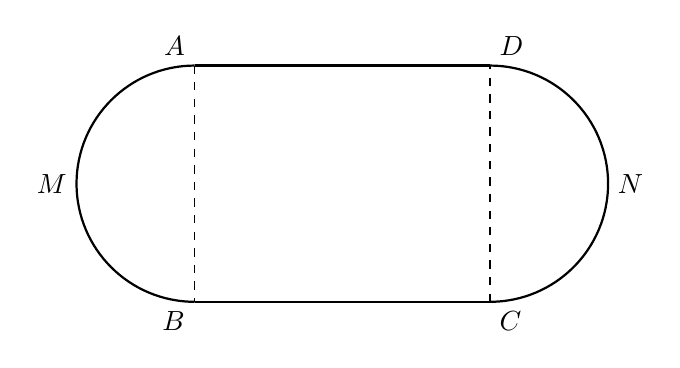
\begin{tikzpicture}[scale=1.5]
    \coordinate (A) at (0, 1);
    \coordinate (B) at (0, -1);
    \coordinate (C) at (2.5, -1);
    \coordinate (D) at (2.5, 1);

    \draw[thick] (A) -- (D);
    \draw[thick] (B) -- (C);

    \draw[dashed] (A) -- (B);
    \draw[dashed] (C) -- (D);

    \draw[thick] (A) arc (90:270:1);
    \draw[thick] (D) arc (90:-90:1);

    \node[above left] at (A) {$A$};
    \node[below left] at (B) {$B$};
    \node[below right] at (C) {$C$};
    \node[above right] at (D) {$D$};

    \node[left] at (-1, 0) {$M$};
    \node[right] at (3.5, 0) {$N$};
  \end{tikzpicture}
\end{figure}

\end{document}
